\documentclass[12pt,a4paper]{article}
\usepackage[utf8]{inputenc}
\usepackage{geometry}
\usepackage{graphicx}
\usepackage{amsmath}
\usepackage{hyperref}
\usepackage{lipsum}
\usepackage{longtable}
\usepackage{booktabs}
\usepackage{indentfirst}

% Page layout
\geometry{top=1in, bottom=1in, left=1in, right=1in}

% Title settings
\begin{document}
\begin{titlepage}
    \centering
    \vspace*{1cm}

    {\LARGE \textbf{Deep Learning Course}}\\[0.5cm]
    {\Large \textbf{Final Project Report}}\\[2cm]

      % Menambahkan logo atau gambar di atas judul
    
\includegraphics[width=0.2\textwidth]{unhass.png} \\[1cm]  % Sesuaikan nama file dan ukuran logo

    % Daftar penulis
    \textbf{Disusun oleh:}\\[0.5cm]
    \begin{tabbing}
        \hspace{4cm} \= Joy Abrian Rantepasang \hspace{1.5cm} \= H071221030 \kill
        \> Joy Abrian Rantepasang \hspace{1cm} \= H071221030 \\
        \> Ahmad Fauzhan Ramadhan \hspace{0.4cm} \= H071221062 \\
        \> Zefanya Farrel Palinggi \hspace{1.25cm} \= H071221070 \\
    \end{tabbing}
    
    \vfill
    
    % Informasi universitas dan tanggal
    \textbf{Universitas Hasanuddin}\\
    \textbf{Makassar, Indonesia}\\[0.5cm]
    \textbf{\today}
    
\end{titlepage}


\tableofcontents
\newpage

\section{Introduction}
\subsection{Background \& Context}

Dataset yang berjudul "Anime Art: AI or Human?" dibuat untuk menangani tantangan yang semakin besar dalam membedakan gambar anime yang dihasilkan oleh AI atau yang dibuat oleh manusia. Seiring dengan pesatnya perkembangan model AI, khususnya GAN (Generative Adversarial Networks) dan model difusi, kemampuan untuk menghasilkan karya seni anime yang realistis dan mendetail semakin meningkat. Perkembangan ini menimbulkan pertanyaan mengenai keaslian, hak cipta, serta dampaknya terhadap seniman manusia. Dataset ini dibuat untuk memberikan sumber daya yang terstruktur bagi peneliti, pengembang, dan penggemar AI dalam melatih serta mengevaluasi model deteksi yang dapat membedakan seni anime buatan AI.

\subsection{Problem Statement}
Seiring dengan kemajuan teknologi AI, semakin sulit untuk membedakan karya seni anime yang dibuat oleh AI dengan karya yang dibuat oleh manusia. Tantangan ini memiliki implikasi di berbagai bidang, termasuk hukum hak cipta, peran pencipta manusia, dan pemahaman lebih luas tentang kreativitas di era AI. Masalah utama yang ingin diatasi oleh dataset ini adalah kebutuhan akan alat yang efektif untuk membedakan keduanya, yang memungkinkan model deteksi yang lebih akurat dan mendorong diskusi mengenai aspek etis dari seni yang dihasilkan oleh AI.

\subsection{Objectives of the Research}
Proyek ini bertujuan untuk:

\begin{enumerate}
   \item Mendukung penelitian AI dengan menyediakan sumber daya yang komprehensif bagi peneliti dan pengembang yang bekerja pada model deteksi, khususnya yang berfokus pada gambar bergaya anime.
        \item Meningkatkan pelatihan model dengan memungkinkan pelatihan yang lebih akurat untuk membedakan gambar anime buatan AI dan manusia, sehingga meningkatkan akurasi dan ketahanan model deteksi.
        \item Mendorong diskusi dan penelitian tentang penggunaan AI yang etis, dengan tujuan menciptakan keseimbangan antara inovasi dan perlindungan kreativitas manusia.
\end{enumerate}
\newpage

% 2. Related Works
\section{Related Works}

\subsection{Literature review of relevant papers and articles.}
Sejumlah penelitian terbaru telah mengembangkan berbagai metode untuk mendeteksi gambar yang dihasilkan oleh AI, terutama yang berfokus pada seni bergaya anime. Salah satu penelitian yang menonjol adalah yang dilakukan oleh para peneliti dalam \textit{Detection of AI-Generated Anime Images Using Deep Learning}. Penelitian ini mengaplikasikan model deep learning berbasis MobileNetV2 dan MobileNetV3 untuk membedakan antara gambar anime yang dihasilkan oleh AI dan gambar yang dibuat oleh manusia. Dengan memanfaatkan transfer learning pada dataset yang berisi gambar-gambar anime dari kedua kategori tersebut, penelitian ini menunjukkan bahwa model deep learning dapat memberikan akurasi yang sangat tinggi dalam melakukan deteksi. Meskipun demikian, penelitian ini juga menyadari adanya keterbatasan dalam hal ukuran dataset yang digunakan, yang dapat memengaruhi kemampuan model untuk mengenali berbagai gaya anime yang berbeda. Selain itu, adanya bias terhadap gaya tertentu dalam gambar anime juga menjadi tantangan yang belum sepenuhnya teratasi dalam penelitian ini.

Studi lain yang relevan adalah \textit{Online Detection of AI-Generated Images}, yang berfokus pada deteksi gambar AI secara daring. Penelitian ini memanfaatkan pelatihan progresif dengan menggunakan dataset besar yang mencakup gambar-gambar dari 14 model generatif yang berbeda. Pendekatan ini memungkinkan model untuk beradaptasi secara bertahap dengan model-model AI generatif baru, mencapai akurasi deteksi yang tinggi. Namun, penelitian ini menghadapi kesulitan dalam mendeteksi gambar yang dihasilkan oleh model-model eksklusif atau model yang tidak terbuka, yang semakin banyak bermunculan. Tantangan ini menunjukkan bahwa meskipun model deteksi daring dapat menangani sejumlah besar gambar, kemampuan mereka untuk menangani model AI yang lebih baru atau jarang terbuka masih terbatas.

Selain itu, dalam \textit{Detection of AI-Created Images Using Pixel-Wise Feature Extraction and CNN}, penelitian ini mengembangkan pendekatan berbasis ekstraksi fitur per piksel untuk mendeteksi gambar yang dihasilkan oleh AI. Teknik seperti Photo Response Non-Uniformity (PRNU) dan Error Level Analysis (ELA) dikombinasikan dengan Convolutional Neural Networks (CNN) untuk meningkatkan akurasi deteksi. Hasil penelitian ini menunjukkan bahwa pendekatan ini mampu membedakan gambar AI dari gambar asli dengan akurasi lebih dari 95\%.  Namun, tantangan utama yang dihadapi oleh metode ini adalah kemampuan model untuk mengatasi variasi gambar yang dihasilkan melalui proses post-processing, yang dapat mengubah karakteristik gambar AI sehingga sulit dikenali oleh model.

Sementara itu, pendekatan zero-shot yang digunakan dalam \textit{Zero-Shot Detection of AI-Generated Images} menawarkan sebuah inovasi dengan mendeteksi gambar AI tanpa perlu pelatihan model pada dataset gambar yang spesifik. Metode ini mengandalkan model bahasa besar yang disesuaikan untuk mendeteksi gambar, dengan fokus pada metrik seperti negative log-likelihood dan entropy. Pendekatan ini menunjukkan hasil yang menjanjikan dalam mendeteksi berbagai jenis gambar AI, meskipun masih terdapat ruang untuk perbaikan, terutama dalam mendeteksi gambar dari model-model AI yang belum pernah dilihat sebelumnya. Kemampuan untuk mendeteksi gambar tanpa pelatihan khusus pada model generatif tertentu membuka potensi besar untuk aplikasi deteksi yang lebih luas, namun memerlukan lebih banyak penelitian untuk meningkatkan akurasi pada model-model yang lebih eksperimental.

Terakhir, penelitian \textit{GenImage: A Million-Scale Benchmark for Detecting AI-Generated Images} mengintroduksi dataset besar yang berfungsi sebagai benchmark untuk mengevaluasi detektor gambar AI dari berbagai model, termasuk GANs dan model difusi. GenImage berisi lebih dari satu juta gambar, yang memungkinkan evaluasi menyeluruh atas kinerja model deteksi dalam mengenali gambar dari berbagai model generatif. Meskipun dataset ini berhasil mendeteksi gambar dalam jenis model yang sama, tantangan utama yang dihadapi adalah dalam hal generalisasi lintas model. Model deteksi yang telah dilatih pada satu jenis model generatif belum tentu efektif dalam mendeteksi gambar yang dihasilkan oleh model generatif lain yang berbeda.

Dari berbagai penelitian tersebut, dapat disimpulkan bahwa meskipun berbagai metode deteksi gambar AI telah berhasil dikembangkan, tantangan utama yang masih dihadapi adalah masalah generalisasi dan adaptasi terhadap model AI yang baru dan beragam. Oleh karena itu, penelitian ini bertujuan untuk mengembangkan model deteksi yang lebih fleksibel dan robust dengan memanfaatkan teknik deep learning yang telah terbukti efektif, sambil mempertimbangkan keberagaman gaya gambar anime dan kemampuan deteksi lintas model.


 \subsection{Comparison of different approaches and their results.}Beberapa pendekatan yang telah digunakan untuk mendeteksi gambar yang dihasilkan oleh AI menunjukkan kekuatan dan keterbatasan masing-masing. Model berbasis deep learning, seperti yang digunakan dalam \textit{Detection of AI-Generated Anime Images Using Deep Learning}, memiliki akurasi tinggi tetapi tergantung pada ukuran dataset dan keberagaman gaya anime yang digunakan. Di sisi lain, pendekatan seperti \textit{Zero-Shot Detection of AI-Generated Images} menawarkan keuntungan dalam hal fleksibilitas dan kemampuan mendeteksi gambar yang dihasilkan oleh model-model yang belum dikenal. Namun, pendekatan ini masih memerlukan penyempurnaan untuk mencapai kinerja yang optimal pada model-model yang lebih baru.

Pendekatan berbasis fitur per piksel, seperti yang digunakan dalam \textit{Detection of AI-Created Images Using Pixel-Wise Feature Extraction and CNN}, menunjukkan hasil yang sangat baik dalam membedakan gambar AI dari gambar asli dengan akurasi lebih dari 95\%. Namun, metode ini menghadapi tantangan dalam mengatasi variasi gambar yang dihasilkan melalui post-processing. Sementara itu, dataset besar seperti \textit{GenImage} menawarkan potensi untuk meningkatkan generalisasi dan akurasi deteksi di berbagai model, meskipun tantangan dalam generalisasi lintas model tetap menjadi hambatan.

\subsection{Justification for Your Chosen Methodology:}

Pemilihan metodologi dalam proyek ini didasarkan pada sejumlah pertimbangan untuk memastikan efektivitas model dalam tugas klasifikasi gambar. Model VGG16 dipilih karena arsitekturnya yang dalam dan terbukti efektif dalam mengatasi tugas-tugas pengenalan citra, serta kemampuannya untuk mengekstraksi fitur dari gambar dengan berbagai tingkat kompleksitas. Meskipun kami melatih model VGG16 dari awal tanpa menggunakan bobot pretrained, pendekatan ini memberikan kesempatan bagi model untuk belajar langsung dari dataset yang relevan dengan tugas ini, meskipun bisa menghadapi tantangan seperti underfitting. Selain itu, kami menggunakan teknik \textit{data augmentation} untuk menghasilkan variasi tambahan pada gambar, yang membantu mengatasi masalah overfitting serta meningkatkan generalisasi model, terutama pada dataset yang terbatas. Mengingat kemungkinan ketidakseimbangan kelas dalam dataset, kami juga menggunakan \textit{class weights} untuk memberikan bobot lebih pada kelas yang kurang terwakili, guna meningkatkan presisi dan recall pada kelas tersebut. Evaluasi model menggunakan metrik yang relevan seperti akurasi, presisi, recall, dan F1-score memberikan gambaran yang lebih komprehensif tentang kinerja model, terutama dalam konteks ketidakseimbangan kelas. F1-score, yang merupakan rata-rata harmonis antara presisi dan recall, sangat berguna untuk menilai kinerja model secara keseluruhan, terutama ketika kesalahan dalam klasifikasi kelas tertentu harus diminimalkan. Penggunaan confusion matrix juga dipilih untuk menganalisis kesalahan spesifik pada kelas tertentu, yang memungkinkan perbaikan lebih lanjut dalam model, seperti penanganan kelas yang sulit dikenali. Dengan pendekatan ini, metodologi yang dipilih diharapkan dapat memberikan pemahaman yang lebih baik dan hasil yang optimal dalam klasifikasi gambar.


\newpage

\section{Dataset and Material}
Pada proyek ini, kami menggunakan dataset yang berfokus pada gambar anime yang dihasilkan oleh AI dan gambar anime yang dibuat oleh manusia. Berikut adalah rincian dari dataset yang digunakan:

\subsection{Source of the dataset:}
Dataset gambar AI diambil dari TWDNE (The World's Database of Non-Existent Art), sementara dataset gambar manusia diperoleh dari \href{https://www.kaggle.com/datasets/splcher/animefacedataset}{AnimeFaceDataset} yang tersedia di Kaggle. Kedua dataset ini dipilih karena keduanya berfokus pada gambar anime yang dapat membedakan dengan jelas antara gambar yang dihasilkan oleh AI dan gambar yang dibuat oleh manusia.

\begin{table}[h!]
\centering
\begin{tabular}{|c|c|}
\hline
\textbf{Dataset} & \textbf{Jumlah Dataset} \\
\hline
AI-generated images & 10938 \\
\hline
Human-generated images & 10938\\
\hline
\end{tabular}
\caption{Rincian Jumlah dataset yang digunakan}
\label{table:dataset_sources}
\end{table}

    
\subsection{Preprocessing Steps}.

Pada proyek ini, beberapa langkah preprocessing dilakukan untuk mempersiapkan dataset sebelum digunakan dalam pelatihan model dan analisis lebih lanjut. Berikut adalah rangkuman dari langkah-langkah preprocessing yang dilakukan:


\begin{itemize}
    \item \textbf{Pemrosesan Dataset dan Struktur Direktori}
    Dataset dibagi menjadi dua direktori utama: \texttt{train} dan \texttt{test}, yang masing-masing berisi subdirektori untuk kategori \texttt{human-art} dan \texttt{ai-generated}. Gambar-gambar diatur sesuai dengan kategori ini dan direktori tersebut diakses melalui Google Drive untuk mempermudah pengelolaan data.

\item \textbf{Penghitungan Gambar dan Distribusi Kelas}
    Untuk memahami distribusi gambar di setiap kategori, dilakukan penghitungan jumlah gambar pada setiap kategori dalam dataset pelatihan dan pengujian. Langkah ini membantu untuk mengetahui jika terdapat ketidakseimbangan kelas, yang bisa mempengaruhi pelatihan model. Distribusi ini divisualisasikan dalam bentuk grafik batang untuk menunjukkan jumlah gambar di masing-masing kategori.

\newpage
\item \textbf{Analisis Ukuran Gambar}.
    Gambar-gambar pada dataset pelatihan dianalisis untuk mengetahui dimensi (lebar dan tinggi) gambar. Langkah ini dilakukan untuk mengevaluasi apakah terdapat variasi ukuran gambar yang signifikan yang mungkin memerlukan penyesuaian ukuran (resizing) atau normalisasi. Distribusi lebar dan tinggi gambar divisualisasikan untuk memahami variabilitas dataset. Hasil analisis menunjukkan bahwa ukuran gambar relatif konsisten, sehingga tidak diperlukan langkah resizing.

     \begin{figure}[h]
        \centering
        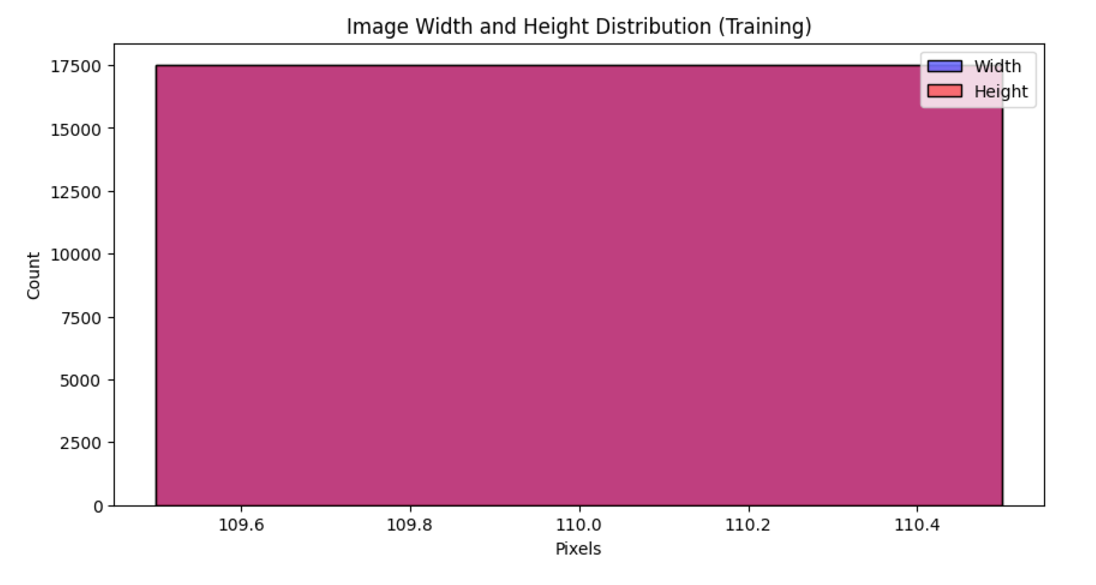
\includegraphics[width=0.5\textwidth, height=5cm]{size.png}  % Ganti dengan path gambar Anda
        \caption{Image Size Analysis}
    \end{figure}

\item \textbf{Pemeriksaan Sampel Gambar}.
    Beberapa gambar sampel dari setiap kategori ditampilkan untuk melakukan inspeksi visual terhadap dataset. Langkah ini memberikan gambaran umum mengenai kualitas gambar dan memastikan bahwa dataset memiliki gambar dari kedua kategori yang cukup representatif dan berbeda secara visual, sehingga dapat digunakan untuk tugas klasifikasi.

\item \textbf{Analisis Warna}.
    Dilakukan analisis terhadap nilai rata-rata RGB dari setiap gambar untuk memeriksa distribusi warna dalam dataset pelatihan. Nilai rata-rata intensitas untuk saluran merah, hijau, dan biru dihitung dan divisualisasikan. Langkah ini membantu untuk memahami karakteristik warna dari gambar, yang mungkin berguna dalam membedakan dua kategori, \texttt{human-art} dan \texttt{ai-generated}.

    \begin{figure}[h]
        \centering
        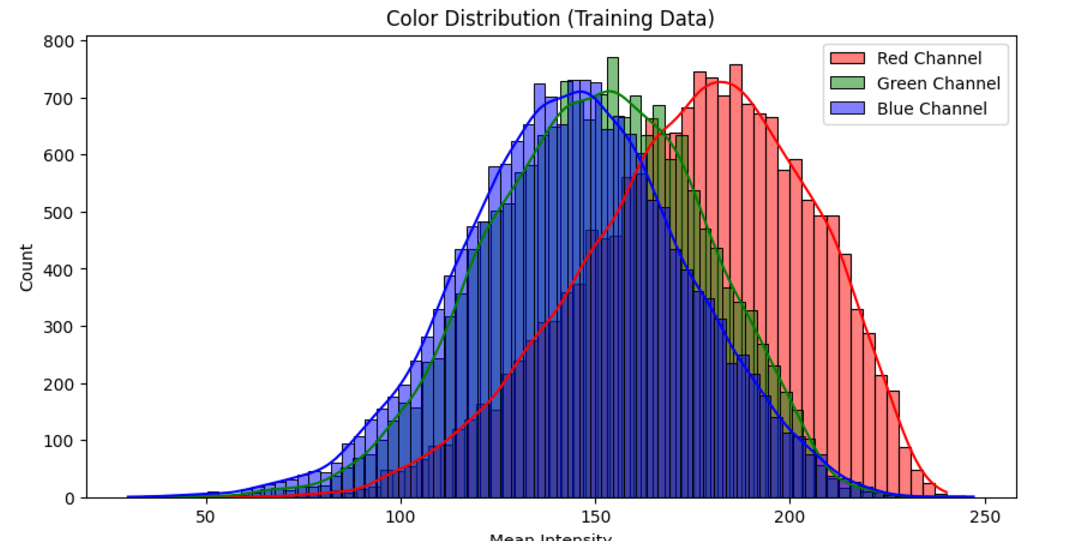
\includegraphics[width=0.5\textwidth, height=5cm]{color.png}  % Ganti dengan path gambar Anda
        \caption{Color Analysis}
    \end{figure}
    \end{itemize}
    
\subsection{Features and labels included in the data}

Pada dataset ini, terdapat dua kategori utama yang ingin dibedakan: \texttt{human-art} dan \texttt{ai-generated}. Berikut adalah penjelasan mengenai fitur-fitur yang ada dalam dataset dan label yang ingin diprediksi.

\subsubsection{Fitur (Features)}
    Fitur-fitur dalam dataset ini merujuk pada atribut atau informasi yang digunakan untuk membedakan antara gambar dari kategori \texttt{human-art} dan \texttt{ai-generated}. Beberapa fitur yang relevan yang dapat diekstrak dari gambar antara lain:

\begin{itemize}
    \item \textbf{Dimensi Gambar (Image Dimensions)}: Ukuran gambar, termasuk lebar dan tinggi, yang dapat mempengaruhi fitur visual dari gambar. Meskipun gambar dalam dataset ini relatif konsisten dalam hal ukuran, fitur ini dapat digunakan dalam beberapa kasus untuk analisis lebih lanjut.
    
    \item \textbf{Warna (Color)}: Rata-rata nilai RGB dari setiap gambar, yang menunjukkan dominasi warna dalam gambar. Fitur warna ini bisa membantu dalam membedakan antara seni yang dibuat oleh manusia dan seni yang dihasilkan oleh AI, karena keduanya mungkin memiliki karakteristik warna yang berbeda.
    
    \item \textbf{Tekstur dan Pola (Texture and Patterns)}: Meskipun tidak diekstrak secara eksplisit dalam dataset ini, fitur seperti tekstur dan pola dalam gambar bisa menjadi indikator penting yang membedakan antara karya seni manusia dan AI, yang dapat dianalisis lebih lanjut menggunakan metode pemrosesan citra.
\end{itemize}
  
\subsubsection{Label (Labels)}
    Label dalam dataset ini adalah variabel yang ingin diprediksi oleh model. Label yang ada dalam dataset ini menunjukkan apakah gambar tersebut termasuk dalam kategori \texttt{human-art} atau \texttt{ai-generated}. Dengan kata lain, label ini adalah target klasifikasi yang digunakan untuk melatih model pembelajaran mesin untuk mengklasifikasikan gambar berdasarkan asal-usulnya:
    \begin{figure}[h]
        \centering
        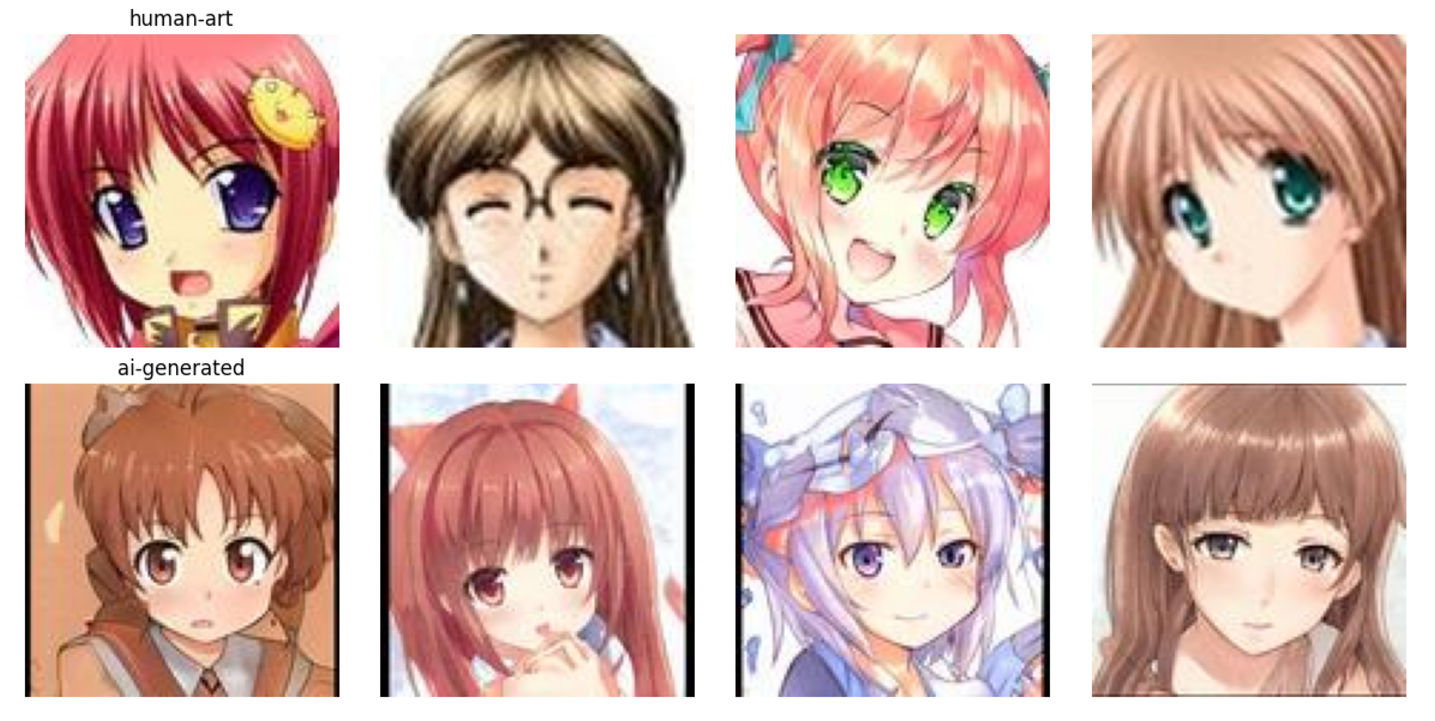
\includegraphics[width=0.4\textwidth]{anime.png}  % Ganti dengan path gambar Anda
        \caption{Contoh gambar \texttt{human-art dan AI-Generates}}
    \end{figure}
    
\newpage
% 4. Result and Discussion
\section{Result And Discussion}
Pada evaluasi model, metrik kinerja yang diperoleh adalah sebagai berikut: \textbf{Akurasi} sebesar 50.00\%, \textbf{Presisi} 25.00\%, \textbf{Recall} 50.00\%, dan \textbf{F1-Score} 33.33\%. Metrik-metrik ini menunjukkan bahwa model memiliki recall yang moderat, tetapi presisi dan F1-score yang relatif rendah. Hal ini mungkin disebabkan oleh masalah seperti ketidakseimbangan kelas atau underfitting pada model. Untuk memberikan gambaran yang lebih jelas, berikut ditampilkan Confusion Matrix, yang menggambarkan bagaimana prediksi model dibandingkan dengan label yang sebenarnya. Matriks ini menunjukkan bahwa beberapa kelas lebih sering diklasifikasikan dengan salah, yang dapat menjelaskan nilai presisi yang rendah pada beberapa kelas. Selain itu, performa model juga divisualisasikan melalui grafik kurva presisi-recall atau plot akurasi, yang dapat membantu mengidentifikasi area yang perlu diperbaiki. Mengingat presisi yang relatif rendah, langkah-langkah seperti fine-tuning model atau menangani ketidakseimbangan kelas mungkin dapat meningkatkan performa model lebih lanjut.

\begin{figure}[h!]
    \centering
    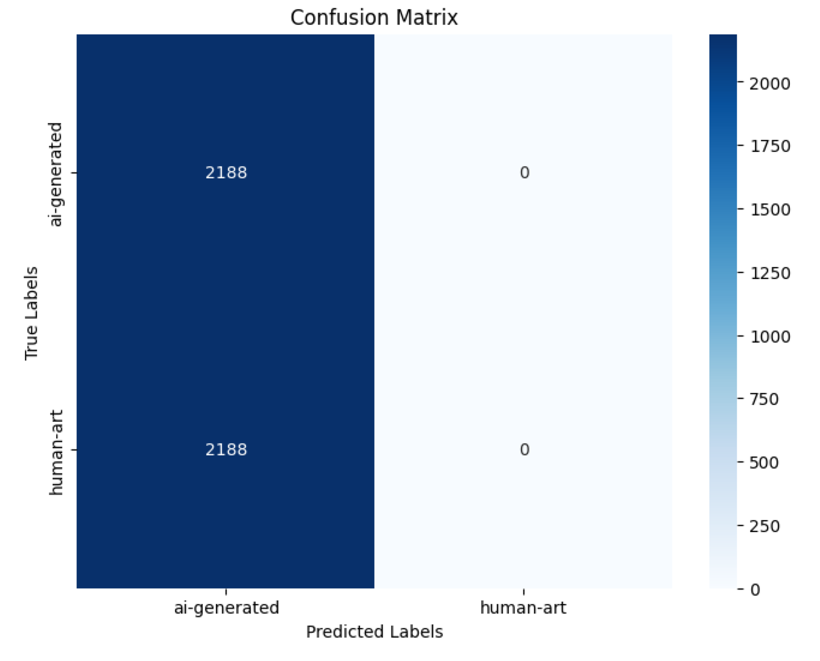
\includegraphics[width=0.8\textwidth]{confus.png} % Ganti dengan gambar matriks kebingungannya Anda
    \caption{Confusion Matrix untuk Evaluasi Model}
    \label{fig:confusion_matrix}
\end{figure}
    
\subsection{Discussion of the Result}

Berdasarkan hasil evaluasi model, metrik kinerja yang diperoleh menunjukkan bahwa model masih memiliki beberapa kelemahan dalam hal presisi dan F1-score. Meskipun akurasi model mencapai 50.00\%, yang berarti model dapat mengenali setengah dari data dengan benar, presisi yang hanya 25.00\% menunjukkan bahwa model sering membuat prediksi yang salah pada beberapa kelas. Hal ini dapat dilihat pada matriks kebingungannya, yang menunjukkan bahwa model kesulitan dalam membedakan antara beberapa kategori gambar. Terutama pada kelas yang kurang terwakili dalam dataset, model cenderung lebih sering salah mengklasifikasikan gambar.

F1-score yang rendah (33.33\%) mengindikasikan bahwa meskipun model memiliki recall yang moderat, ketidakseimbangan antara presisi dan recall mengarah pada performa yang suboptimal dalam deteksi kelas tertentu. Recall sebesar 50.00\% menunjukkan bahwa model mampu mendeteksi setengah dari gambar dalam kelas yang benar, tetapi kurang baik dalam menghindari kesalahan deteksi untuk beberapa kelas lainnya.

Masalah ketidakseimbangan kelas dapat menjadi faktor utama penyebab rendahnya presisi dan F1-score. Jika dataset memiliki distribusi kelas yang tidak seimbang, model cenderung memprediksi kelas yang lebih dominan dengan lebih akurat, sementara kelas yang lebih sedikit terwakili dapat lebih sering salah diklasifikasikan. Hal ini mungkin yang terjadi pada model ini, di mana beberapa kelas kurang terwakili dalam dataset dan model cenderung mengabaikan atau salah mengklasifikasikan gambar-gambar dari kelas tersebut.

Selain itu, hasil ini bisa juga disebabkan oleh masalah \textit{underfitting}, di mana model mungkin belum cukup dilatih untuk menangkap pola yang lebih kompleks dalam data. Pelatihan lebih lanjut dengan data yang lebih banyak, penggunaan augmentasi data, atau fine-tuning model dengan menggunakan bobot pretrained dari model yang sudah dilatih pada dataset yang lebih besar dapat menjadi solusi untuk memperbaiki hasil ini.

Untuk meningkatkan performa model, langkah-langkah seperti penanganan ketidakseimbangan kelas, baik dengan cara \textit{data augmentation} atau penggunaan \textit{class weights}, bisa dicoba. Selain itu, eksperimen dengan arsitektur model yang lebih kompleks atau menggunakan model pretrained seperti VGG16 atau ResNet dengan fine-tuning juga bisa meningkatkan akurasi dan mengurangi kesalahan klasifikasi.

Secara keseluruhan, meskipun model menunjukkan hasil yang moderat, perbaikan di area yang telah disebutkan dapat meningkatkan kemampuan model dalam mengenali gambar dengan lebih baik dan mengatasi masalah yang ada pada kelas yang kurang terwakili.

\newpage
% 5. Conclusion
\section{Conclusion}

Proyek ini bertujuan untuk mengembangkan model deep learning yang dapat membedakan antara gambar anime yang dihasilkan oleh AI dan gambar yang dibuat oleh manusia. Tujuan utama penelitian ini adalah untuk menyediakan sumber daya yang berguna bagi peneliti dan pengembang dalam menghadapi tantangan deteksi gambar AI. Berdasarkan hasil yang diperoleh, model menunjukkan kinerja moderat dengan akurasi 50.00\%, recall 50.00\%, namun presisi dan F1-score yang relatif rendah. Meskipun demikian, hasil ini memberikan wawasan yang penting mengenai tantangan yang dihadapi dalam klasifikasi gambar anime, terutama terkait dengan masalah ketidakseimbangan kelas dan underfitting.

Beberapa temuan utama dari proyek ini adalah:
\begin{itemize}
    \item \textbf{Kemampuan moderat model}: Model memiliki kemampuan moderat untuk mengenali gambar dari kedua kategori, tetapi mengalami kesulitan dalam mengklasifikasikan gambar-gambar yang kurang terwakili dalam dataset.
    \item \textbf{Presisi rendah}: Metrik presisi yang rendah menunjukkan bahwa model sering kali membuat kesalahan dalam mengklasifikasikan gambar, yang bisa disebabkan oleh distribusi kelas yang tidak seimbang.
    \item \textbf{Recall lebih baik daripada presisi}: Recall yang lebih baik daripada presisi menunjukkan bahwa model mampu mendeteksi gambar-gambar yang relevan, tetapi dengan banyak kesalahan dalam proses klasifikasi.
\end{itemize}

Sebagai langkah perbaikan, disarankan untuk:
\begin{itemize}
    \item \textbf{Meningkatkan dataset}: Menambah variasi dan jumlah gambar, serta menangani ketidakseimbangan kelas baik dengan data augmentation atau penggunaan class weights.
    \item \textbf{Fine-tuning dengan model pretrained}: Melakukan fine-tuning dengan model pretrained untuk memperbaiki underfitting dan meningkatkan generalisasi.
    \item \textbf{Mencoba arsitektur model yang lebih kompleks}: Mencoba arsitektur model yang lebih kompleks, seperti menggunakan model ResNet atau EfficientNet, untuk meningkatkan akurasi deteksi.
\end{itemize}

Secara keseluruhan, meskipun hasil yang diperoleh belum optimal, penelitian ini memberikan landasan yang baik untuk pengembangan model yang lebih akurat dalam mendeteksi gambar yang dihasilkan oleh AI. Penelitian lebih lanjut dengan dataset yang lebih besar dan beragam serta teknik pelatihan yang lebih lanjut akan sangat bermanfaat untuk mencapai hasil yang lebih baik.

\newpage
\section*{References}
\bibliographystyle{plain}
Cozzolino, D., Poggi, G., Nießner, M., & Verdoliva, L. (n.d.). Zero-Shot Detection of AI-Generated Images.

Epstein, D. C., Jain, I., Wang, O., & Zhang, R. (n.d.). Online Detection of AI-Generated Images.

Kusuma, S. W., Natalia, F., Ko, C. S., & Sudirman, S. (2023, September). DETECTION OF AI-GENERATED ANIME IMAGES USING DEEP LEARNIN. ICIC Express Letters Part B: Applications.

Zhu, M., Zhen, H., Yan, Q., & Huang, X. (n.d.). GenImage: A Million-Scale Benchmark for Detecting AI-Generated Image.



\end{document}